\newpage % Rozdziały zaczynamy od nowej strony.
\section{Wstęp}
Zagadnieniem systemów komunikacji człowiek zajmuje się już od XIX w. Rozwój systemów komunikacji wiąże się, z rozwojem wielu dziedzin techniki i nauki na niespotykaną do tej pory skalę. Problemy komunikacji na odległość i ich rozwiązania zajmują najtęższe umysły od prawie 200 lat. Przykładem a zarazem pierwszym urządzeniem komunikacyjnym jest telegraf\cite{wiki:telegraf2023}.
W odpowiedzi na potrzeby i różnego rodzaju wymagania powstały liczne dedykowane systemy komunikacyjne i urządzenia z nich korzystające.
Większość obecnie dostępnych systemów komunikacji wymaga dostępu do jakiejś sieci np. GSM(telefonia komórkowa, w tym MMS-y i SMS-y), Internet(popularne komunikatory takie jak np. Whatsapp, Signal lub Telegram).
Istotnym więc dla tej pracy dyplomowej stało się wytworzenie systemu komunikacyjnego, który działał by niezależnie od dostępności do [jakiejkolwiek] sieci - co czyniłoby go idealnym rozwiązaniem w sytuacjach kryzysowych.
Wytworzone rozwiązanie oparte jest w dużej mierze na rozwiązaniach otwartych, co umożliwia jego dostosowanie do szczególnych wymogów.
\begin{figure}[!h]
	\centering 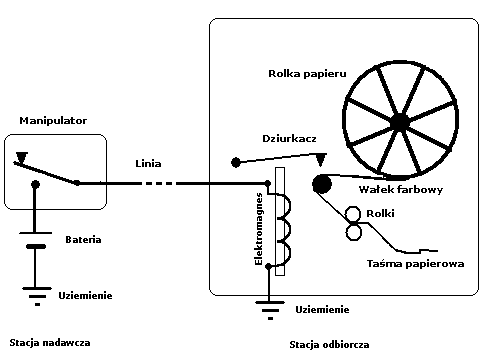
\includegraphics[width=0.5\linewidth]{telegraf.png}
	\caption{Schemat telegrafu. Źródło: wikipedia}
	\label{fig:telegraf}
\end{figure}
\subsection{Cele pracy}
Do celów niniejszej pracy należy:
\begin{itemize}
	\item zaprojektowanie, wykonanie i przetestowanie systemu do komunikacji tekstowej wykorzystującej protokół Lora,
	\item przygotowanie dedykowanej aplikacji mobilnej do obsługi tego systemu,
	\item przygotowanie dokumentacji technicznej,
	\item zaprojektowanie i montaż dedykowanej obudowy do części systemu wykorzystującej mikrokontroler,
	\item zbadanie efektywności stworzonego rozwiązania (ze względu na maksymalny dystans, przy którym komunikacja będzie jeszcze możliwa)
\end{itemize}